% This file was created by matlab2tikz.
%
%The latest updates can be retrieved from
%  http://www.mathworks.com/matlabcentral/fileexchange/22022-matlab2tikz-matlab2tikz
%where you can also make suggestions and rate matlab2tikz.
%
\documentclass[tikz]{standalone}
\usepackage[T1]{fontenc}
\usepackage[utf8]{inputenc}
\usepackage{pgfplots}
\usepackage{grffile}
\pgfplotsset{compat=newest}
\usetikzlibrary{plotmarks}
\usepgfplotslibrary{patchplots}
\usepackage{amsmath}
\usetikzlibrary{decorations.markings}
\begin{document}
		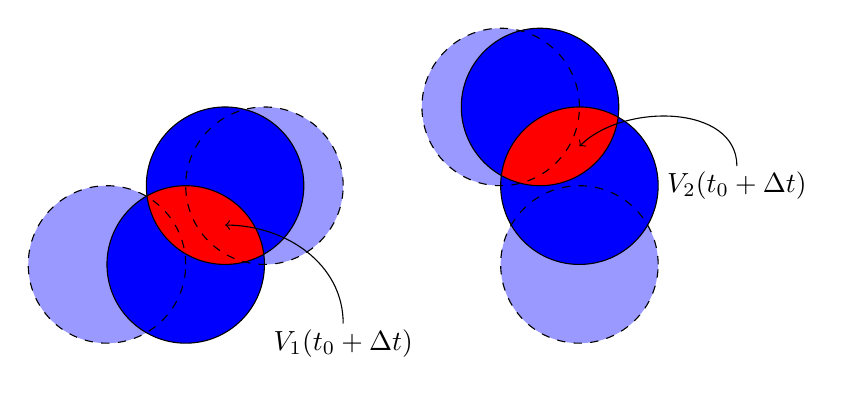
\begin{tikzpicture}[scale=1]
		\fill[blue!40!white](-1,0)circle(1);
		\fill[blue!40!white](1,1)circle(1);
		 \fill[blue](0,0)circle(1);
		\fill[blue](0.5,1)circle(1);
		\begin{scope}
			\clip (0,0) circle(1);
			\fill[red](0.5,1) circle(1);
		\end{scope}
		\draw[dashed](-1,0)circle(1);
		\draw[dashed](1,1)circle(1);
		\draw(0,0)circle(1);
		\draw(0.5,1)circle(1);

		\draw(2,-1)node{$V_1(t_0+\Delta t)$};
		\path[->,draw=black](2,-0.75) to [out=90, in=0](0.5,0.5);
		
		\fill[blue!40!white](4,2)circle(1);
		\fill[blue!40!white](5,0)circle(1);
		 \fill[blue](4.5,2)circle(1);
		\fill[blue](5,1)circle(1);
		\begin{scope}
			\clip (4.5,2) circle(1);
			\fill[red](5,1) circle(1);
		\end{scope}
		\draw[dashed](4,2)circle(1);
		\draw[dashed](5,0)circle(1);
		\draw(4.5,2)circle(1);
		\draw(5,1)circle(1);
		
		\draw(7,1)node{$V_2(t_0+\Delta t)$};
		\path[->,draw=black](7,1.25) to [out=90, in=45](5,1.5);
\end{tikzpicture}
\end{document}